\documentclass[a4paper, 12pt]{article}		% General format
%\documentclass[a4paper, 14pt]{extarticle} % Advanced format

%%%% Charset
\usepackage{cmap}							% Make PDF files searchable and copyable
\usepackage[utf8x]{inputenc}				% Accept different input encodings
\usepackage[T2A]{fontenc}					% Russian font
\usepackage[russian]{babel}					% Multilingual support (T2A)

%%%% Graphics
\usepackage[dvipsnames]{xcolor}			% Driver-independent color extensions
\usepackage{graphicx}						% Enhanced support for graphics
\usepackage{wrapfig}						% Produces figures which text can flow around

%%%% Graphs
\usepackage{tikz}							% Creating graphics programmatically
\usetikzlibrary{arrows}						% Arrows for tikz

%%%% Math
\usepackage{amsmath}						% American Mathematical Society (AMS) math facilities
\usepackage{amsfonts}						% fonts from the AMS
\usepackage{amssymb}						% additional math symbols

%%%% Typography (don't forget about cm-super)
\usepackage{microtype}						% subliminal refinements towards typographical perfection
\linespread{1.3}							% line spacing
\usepackage[left=2.5cm, right=1.5cm, top=2.5cm, bottom=2.5cm]{geometry}
\setlength{\parindent}{0pt}					% we don't want any paragraph indentation
\usepackage{parskip}						% add distance between paragraphs

%%%% Tables
\usepackage{tabularx}						% Enhanced tables
\usepackage{multirow}						% For tabular
\usepackage{hhline}							% For tabular

%%%% Other
\usepackage{url}							% Verbatim with URL-sensitive line breaks
\usepackage{fancyvrb}						% Sophisticated verbatim text
\setcounter{secnumdepth}{5}					% Turn on subsection numbering

%------------------------------------------------------------------------------
\usepackage{listings}						% typeset source code listings

% Цвета для кода
\definecolor{mygreen}{HTML}{3F7F5F} 		% color values Red, Green, Blue
\definecolor{mylilas}{RGB}{170,55,241}

% Настройки отображения кода
\lstset{language=Matlab,%
    %basicstyle=\color{red},
    breaklines=true,						% Перенос длинных строк
    morekeywords={matlab2tikz},
    keywordstyle=\color{blue},%
    morekeywords=[2]{1}, keywordstyle=[2]{\color{black}},
    identifierstyle=\color{black},%
    stringstyle=\color{mylilas},
    commentstyle=\color{mygreen},%
    showstringspaces=false,					% don't mark spaces in strings
    frame=tblr								% draw a frame at all sides of the code block
	rulecolor=\color{frame},				% Цвет рамки
	tabsize=2,								% tab space width
	showstringspaces=false,					% don't mark spaces in strings
    numbers=left,%
    numberstyle={\tiny \color{black}},% size of the numbers
    numbersep=9pt, % this defines how far the numbers are from the text
    emph=[1]{for,end,break},emphstyle=[1]\color{red}, %some words to emphasise
    %emph=[2]{word1,word2}, emphstyle=[2]{style},    
	% Для отображения русского языка
	extendedchars=true,
	literate=
		{Ö}{{\"O}}1						{Ä}{{\"A}}1						{Ü}{{\"U}}1
		{ß}{{\ss}}1						{ü}{{\"u}}1						{ä}{{\"a}}1
		{ö}{{\"o}}1						{~}{{\textasciitilde}}1			{а}{{\selectfont\char224}}1
		{б}{{\selectfont\char225}}1		{в}{{\selectfont\char226}}1		{г}{{\selectfont\char227}}1
		{д}{{\selectfont\char228}}1		{е}{{\selectfont\char229}}1		{ё}{{\"e}}1
		{ж}{{\selectfont\char230}}1		{з}{{\selectfont\char231}}1		{и}{{\selectfont\char232}}1
		{й}{{\selectfont\char233}}1		{к}{{\selectfont\char234}}1		{л}{{\selectfont\char235}}1
		{м}{{\selectfont\char236}}1		{н}{{\selectfont\char237}}1		{о}{{\selectfont\char238}}1
		{п}{{\selectfont\char239}}1		{р}{{\selectfont\char240}}1		{с}{{\selectfont\char241}}1
		{т}{{\selectfont\char242}}1		{у}{{\selectfont\char243}}1		{ф}{{\selectfont\char244}}1
		{х}{{\selectfont\char245}}1		{ц}{{\selectfont\char246}}1		{ч}{{\selectfont\char247}}1
		{ш}{{\selectfont\char248}}1		{щ}{{\selectfont\char249}}1		{ъ}{{\selectfont\char250}}1
		{ы}{{\selectfont\char251}}1		{ь}{{\selectfont\char252}}1		{э}{{\selectfont\char253}}1
		{ю}{{\selectfont\char254}}1		{я}{{\selectfont\char255}}1		{А}{{\selectfont\char192}}1
		{Б}{{\selectfont\char193}}1		{В}{{\selectfont\char194}}1		{Г}{{\selectfont\char195}}1
		{Д}{{\selectfont\char196}}1		{Е}{{\selectfont\char197}}1		{Ё}{{\"E}}1
		{Ж}{{\selectfont\char198}}1		{З}{{\selectfont\char199}}1		{И}{{\selectfont\char200}}1
		{Й}{{\selectfont\char201}}1		{К}{{\selectfont\char202}}1		{Л}{{\selectfont\char203}}1
		{М}{{\selectfont\char204}}1		{Н}{{\selectfont\char205}}1		{О}{{\selectfont\char206}}1
		{П}{{\selectfont\char207}}1		{Р}{{\selectfont\char208}}1		{С}{{\selectfont\char209}}1
		{Т}{{\selectfont\char210}}1		{У}{{\selectfont\char211}}1		{Ф}{{\selectfont\char212}}1
		{Х}{{\selectfont\char213}}1		{Ц}{{\selectfont\char214}}1		{Ч}{{\selectfont\char215}}1
		{Ш}{{\selectfont\char216}}1		{Щ}{{\selectfont\char217}}1		{Ъ}{{\selectfont\char218}}1
		{Ы}{{\selectfont\char219}}1		{Ь}{{\selectfont\char220}}1		{Э}{{\selectfont\char221}}1
		{Ю}{{\selectfont\char222}}1		{Я}{{\selectfont\char223}}1		{і}{{\selectfont\char105}}1
		{ї}{{\selectfont\char168}}1		{є}{{\selectfont\char185}}1		{ґ}{{\selectfont\char160}}1
		{І}{{\selectfont\char73}}1		{Ї}{{\selectfont\char136}}1		{Є}{{\selectfont\char153}}1
		{Ґ}{{\selectfont\char128}}1
}

% Для настройки заголовка кода
\usepackage{caption}
\DeclareCaptionFont{white}{\color{сaptiontext}}
\DeclareCaptionFormat{listing}{\parbox{\linewidth}{\colorbox{сaptionbk}{\parbox{\linewidth}{#1#2#3}}\vskip-4pt}}
%\captionsetup[lstlisting]{format=listing,labelfont=white,textfont=white}
\renewcommand{\lstlistingname}{Листинг} % Переименование Listings в нужное именование структуры
%------------------------------------------------------------------------------

\begin{document}

%------------------------------------------------
\begin{titlepage}
\thispagestyle{empty}

\begin{center}
Санкт-Петербургский политехнический университет Петра Великого\\
Институт Информационных Технологий и Управления \\*
Кафедра компьютерных систем и программных технологий \\*
\hrulefill
\end{center}

\vspace{15em}

\begin{center}
\Large Отчёт по практической работе\\по предмету «Системное программное обеспечение» \\
\end{center}

\vspace{1em}

% \linebreak
\begin{center}
\textsc{\textbf{Процесс загрузки операционной системы Linux}}
\end{center}

\vspace{20em}

\begin{flushleft}
Работу выполнил студент гр. 53501/3 \hrulefill Мартынов С. А. \\
\vspace{1.5em}
Работу принял преподаватель \hrulefill Душутина Е. В. \\
\end{flushleft}

\vspace{\fill}

\begin{center}
Санкт-Петербург \\
2015
\end{center}

\end{titlepage}
%------------------------------------------------
\setcounter{page}{2} % Титульная страница
\tableofcontents

%------------------------------------------------------------------------------

\newpage
\section*{Постановка задачи}
\addcontentsline{toc}{section}{Постановка задачи}

\vspace{2em}

В рамках данной работы необходимо ознакомиться приниципами написания драйверов и реализовать драйвер сетевого устройства.

\vspace{1em}

Привести краткую информация о контроллере сетевого устройства и его технические характеристики. Дать описание порядка разработки драйвера и способы взаимодействия ядра с апараторуй. Для используемых структур представить назначение основных полей. Описать взаимодействие драйвера, находящегося в пространстве ядра, с приложениями уровня пользователя.

\vspace{1em}

Сетевое устройство (сетевая карта) может быть выбрана студентом самостоятельно.
 % Постановка задачи

\newpage
\section*{Введение}
\addcontentsline{toc}{section}{Введение}

Драйвер устройства -- это низкоуровневая программа, содержащая специфический код для работы с устройством, которая позволяет пользовательским программам (и самой ОС) управлять им стандартным образом.

В современных версиях ядра Linux по умолчанию присутствуют все необходимые драйверы для всех поддерживаемых устройств\cite{Love}. Но для старых версий ядра иногда приходится заниматься бэк-портированием драйверов или даже написанием из с нуля, чтобы обеспечить корректную работу железа.

Все устройства можно разделить на:
\begin{itemize}
\item \textbf{Символьные}. Чтение и запись устройства идет посимвольно. Примеры таких устройств: клавиатура, последовательные порты.
\item \textbf{Блочные}. Чтение и запись устройства возможны только блоками, обычно по 512 или 1024 байта. Пример - жесткий диск.
\item \textbf{Сетевые интерфейсы}. Отличаются тем, что не отображаются на файловую систему, т.е. не имеют соответствующих файлов в директории /dev, поскольку из-за специфики этих устройств работа с сетевыми устройствами как с файлами неэффективна. Пример - сетевая карта (eth0).
\end{itemize}

В распоряжении имеется относительно старая материнская плата ASUS P5B на чипсете Intel P965, со встроенной сетевой картой на основе Realtek RTL8111B, для которой будет разработан драйвер, работающий в старой версии ядра Linux.

Это довольно популярная платформа r8169, для которой открыта спецификация. Ссылка на неё приводится в списке использованных материалов. % Введение

\newpage
\section{Системные вызовы процессов реального времени}

Для изучения системных вызовов sched\_setparam, sched\_getparam и sched\_rr\_get\_interval целесообразно рассмотреть всю группу системных вызовов, позволяющих процессу менять его дисциплину планирования и, в частности, становиться процессом реального времени. Процесс должен иметь способность CAP\_SYS\_NICE (т.е. способностью изменять приоритет чужих процессов), чтобы модифицировать значения полей rt\_priority и policy у дескриптора любого процесса, включая собственный.

Системный вызов \textbf{sched\_getscheduler} запрашивает политику планирования, действующую в отношении процесса, идентифицируемого параметром pid. Если значение pid во время вызова равен 0, считывается политика вызвавшего процесса. В случае успеха системный вызов возвращает политику sched\_fifo, sched\_rr или sched\_normal (последняя также называется sched\_other). Соответствующая служебная процедура sys\_sched\_getscheduier вызывает функцию find\_process\_by\_pid, которая находит дескриптор процесса по переданному значению pid и возвращает значение его поля policy.

Системный вызов \textbf{sched\_setscheduier} устанавливает как политику планирования, так и соответствующие параметры для процесса, идентифицируемого параметром pid. Как и в случае с sched\_getscheduler, если pid равен 0, то устанавливаются параметры планировщика, применяемые к вызвавшему процессу. Соответствующая служебная процедура sys\_sched\_setscheduler вызывает функцию do\_sched\_setscheduler. Эта функция проверяет допустимость политики планирования, определяемой параметром policy, и нового приоритета, определяемого параметром param->sched\_priority. Она также проверяет, есть ли у процесса способность CAP\_SYS\_NICE, или наличие прав суперпользователя у его владельца. Если все в порядке, она удаляет процесс из очереди на выполнение (если он выполняемый), обновляет статический и динамический приоритеты и приоритет реального времени у процесса, возвращает процесс в очередь на выполнение и, если необходимо, вызывает функцию resched\_task для вытеснения текущего процесса, принадлежащего данной очереди.

Системный вызов \textbf{sched\_getparam} читает параметры процесса, идентифицируемого параметром pid. Если pid равен 0, считываются параметры текущего процесса. Соответствующая служебная процедура sys\_sched\_getparam, как и следует ожидать, находит указатель на дескриптор процесса по параметру
pid, сохраняет поле rt\_priority в локальной переменной типа sched\_param и вызывает функцию copy\_to\_user, чтобы скопировать это значение в адресное пространство процесса, по адресу, заданному параметром param.

Системный вызов \textbf{sched\_setparam} аналогичен вызову sched\_setscheduler, различие состоит в том, что sched\_setparam не позволяет вызвавшему процессу задавать значение поля policy. Соответствующая служебная процедура sys\_sched\_setparam вызывает функцию do\_sched\_setscheduler практически с теми же параметрами, что и служебная процедура sys\_sched\_setscheduler.

Системный вызов \textbf{sched\_yieido} позволяет процессу добровольно освободить процессор без приостановки своего выполнения. Процесс остается в состоянии TASK\_RUNNING, а планировщик заносит его либо в набор процессов с истекшими квантами времени (если это обычный процесс), либо в конец списка в очереди на выполнение (если это процесс реального времени). Затем вызывается функция schedule. В результате у других процессов с тем же динамическим приоритетом появляется возможность поработать. Данный вызов используется, в основном, процессами реального времени, принадлежащими классу SCHED\_FIFO.

Системные вызовы \textbf{sched\_get\_priority\_min} и \textbf{sched\_get\_priority\_max} возвращают, соответственно, минимальный и максимальный статический приоритет реального времени, который может быть использован при проведении политики планирования, идентифицируемой параметром policy. Служебная процедура sys\_sched\_get\_priority\_min возвращает 1, если текущий процесс является процессом реального времени, и 0 в противном случае. Служебная процедура sys\_sched\_get\_priority\_max возвращает 99 (наивысший приоритет), если текущий процесс является процессом реального времени, и 0 в противном случае.

Системный вызов \textbf{sched\_rr\_get\_interval} записывает в структуру, хранящуюся в адресном пространстве режима пользователя, квант времени, соответствующий круговому принципу работы, для процесса реального времени, идентифицируемого параметром pid. Если pid равен 0, системный вызов записывает квант времени текущего процесса. Как и в предыдущих примерах, соответствующая служебная процедура sys\_sched\_rr\_get\_interval вызывает функцию find\_process\_by\_pid, для получения дескриптора процесса по значению pid. Затем она преобразует базовый квант времени выбранного процесса в секунды и наносекунды, и копирует эти числа в структуру пользовательского режима. В соответствии с соглашением, временной квант процесса реального времени, принадлежащего классу "первым вошел — первым вышел", равен нулю.

Рассмотренные системные вызовы позволяют реализовать различные расширения реального времени POSIX.1b начиная с ядра Linux версии 2.6\cite{Raghavan}. Для определения задачи реального времени в Linux есть три основных параметра:
\begin{itemize}
\item Класс планирования
\item Приоритет процесса
\item Интервал времени
\end{itemize}
 
\textbf{Планировщик} Linux предлагает три класса планирования, два для приложений реального времени и один для приложений не реального времени. Этими тремя классами являются:
\begin{itemize}
\item SCHED\_FIFO: политика планирования реального времени первый вошёл, первый вышел (First-In First-Out). Алгоритм планирования не использует никаких интервалов времени. Процесс SCHED\_FIFO выполняется до завершения, если он не заблокирован запросом ввода/вывода, вытеснен высокоприоритетным процессом, или он добровольно отказывается от процессора. Следует обратить внимание на следующие моменты:
\begin{itemize}
\item Процесс SCHED\_FIFO, который был вытеснен другим процессом более высокого приоритета, остаётся во главе списка с его приоритетом и возобновит выполнение, как только все процессы с более высоким приоритетом будут вновь заблокированы.
\item Когда процесс SCHED\_FIFO готов к работе (например, после пробуждения от операции блокировки), он будет вставлен в конец списка с его приоритетом.
\item Вызов sched\_setscheduler или sched\_setparam поставит процесс SCHED\_FIFO в начало списка. Как следствие, это может вытеснить работающий в данный момент процесс, если его приоритет такой же, как и у работающего процесса.
\end{itemize}
\item SCHED\_RR: циклическая (Round-Robin) политика планирования реального времени. Она похожа на SCHED\_FIFO с той лишь разницей, что процессу SCHED\_RR разрешено работать как максимум время кванта. Если процесс SCHED\_RR исчерпывает свой квант времени, он помещается в конец списка с его приоритетом. Процесс SCHED\_RR, который был вытеснен процессом с более высоким приоритетом, завершит оставшуюся часть своего кванта времени после возобновления выполнения.
\item SCHED\_OTHER: стандартный планировщик Linux с разделением времени для процессов, работающих не в реальном времени.
\end{itemize}

Диапазоны \textbf{приоритетов} для различных политик планирования показаны в Таблице 1.

\begin{table}
\caption{Диапазоны приоритетов различных политик планирования}
\centering
\begin{tabular}{|c|c|}
\hline 
Класс планирования & Диапазон приоритетов \\ 
\hline 
SCHED\_OTHER & 0 \\ 
\hline 
SCHED\_FIFO & 1 - 99 \\ 
\hline 
SCHED\_RR & 1 - 99 \\ 
\hline 
\end{tabular}
\end{table}

Ядро позволяет значению nice быть установленным как для процесса SCHED\_RR или SCHED\_FIFO, но это не будет иметь никакого влияния на планирование, пока задача выполняется с классом SCHED\_OTHER.

Точка зрения ядра на приоритеты процессов отличается от точки зрения процессов. Соответствие между приоритетами пользовательского пространства и пространства ядра для задач реального времени в ядре показывает Рисунок 1.

\begin{figure}[h!]
\centering
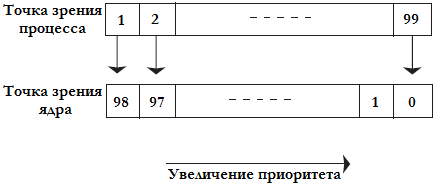
\includegraphics[scale=1]{res/pic001}
\caption{Отображение приоритетов пользовательского уровня на пространство ядра}
\end{figure}

Для ядра низкое значение означает высокий приоритет. Приоритеты реального времени в ядро находятся в диапазоне от 0 до 98. Таким образом, пользовательский приоритет 1 связывается с приоритетом ядра 98, приоритет 2 с 97, и так далее.

\textbf{Интервал времени} действителен только для процессов SCHED\_RR. Процессы SCHED\_FIFO можно рассматривать как имеющие бесконечный интервал времени. Так что это обсуждение касается только процессов SCHED\_RR.

Linux устанавливает минимальный интервал времени для процесса как 10 мс, интервал времени по умолчанию как 100 мс, а максимальный интервал времени как 200 мс. Интервалы времени заполняются вновь после их окончания\cite{Raghavan}. В версии 2.6 интервал времени процесса рассчитывается так:

\begin{Verbatim}[frame=single]
#define MIN_TIMESLICE (10)
#define MAX_TIMESLICE (200)
#define MAX_PRIO (139)   // MAX внутренний приоритет ядра
#define MAX_USER_PRIO 39 // MAX nice при переводе к положительной шкале

/* ‘p’ это структура задач процесса */
#define BASE_TIMESLICE(p) \
   (MIN_TIMESLICE + ((MAX_TIMESLICE - MIN_TIMESLICE) *
   (MAX_PRIO-1 - (p)->static_prio) / (MAX_USER_PRIO-1)))
\end{Verbatim}

Можно заметить, что static\_prio содержит значение nice для процесса. Ядро преобразует диапазон nice c -20 до +19 во внутренний диапазон nice  в ядре от 100 до 139. Поле nice процесса конвертируется в такой масштаб и сохраняется в static\_prio. Таким образом, значение nice -20 соответствует static\_prio 100, а +19 для nice, static\_prio 139. Наконец, интервал времени процесса возвращает функция task\_timeslice.

\begin{Verbatim}[frame=single]
static inline unsigned int task_timeslice(task_t *p) {
  return BASE_TIMESLICE(p);
}
\end{Verbatim}

Отметим, что static\_prio является единственной переменной в расчёте интервала времени. Таким образом, можно сделать некоторые важные выводы:
\begin{itemize}
\item Все процессы SCHED\_RR выполняются по умолчанию с интервалом времени в 100 мс, поскольку они обычно имеют значение nice, равное 0.
\item При значении nice -20 процесс SCHED\_RR получит интервал времени 200 мс, а при nice +19 процесс SCHED\_RR получит  интервал времени 10 мс. Таким образом, значение nice может быть использовано для управления выделением интервала времени для процессов SCHED\_RR.
\item Чем меньше значение nice (то есть, приоритет более высокий), тем больше интервал времени.
\end{itemize}
  % Системные вызовы процессов реального времени

\newpage
\section{Реализация системных вызовов в различных версиях ядра}

Процессы реального времени Linux добавляют новый уровень к схеме приоритетов. Приоритет реального времени хранится в члене rt\_priority структуры struct task\_struct и является целым числом в диапазоне от 0 до 99. (Значение, равное 0, означает, что процесс не является процессом реального времени, и в этом случае его членом policy должен быть SCHED\_OTHER.)

Задачи реального времени используют тот же член counter, что и их аналоги не реального времени, и поэтому их динамические приоритеты обрабатываются таким же образом. Задачи реального времени даже используют член priority для той же цели, что и задачи не реального времени -- в качестве значения, посредством которого они пополняют значение counter, когда оно полностью использовано. Член priority используется только для ранжирования процессов реального относительно друг друга, в остальных случаях они обрабатываются идентично процессам не реального времени.

Поле rt\_priority процесса устанавливается в качестве части определения его политики планирования с помощью стандартизованных POSIX.1b функций sched\_setscheduler и sched\_setparam (которые, обычно, имеет право вызывать только привилегированный пользователь, как будет показано при рассмотрении возможностей). Это означает, что политика планирования процесса может изменяться во время его существования, если, конечно, процесс имеет разрешение выполнять изменение.

Интерфейс изучаемых системных вызовов оказался идентичным (с точностью до смещения строк) для рассматриваемых ядер, поэтому остановимся подробнее на одном из них (2.6). Листинг файла unistd достаточно объёмный и по этой причине не приведён в отчёте.

Системные вызовы, реализующие функции POSIX sched\_setscheduler (строка 27688) и sched\_setparam (строка 27694), делегируют всю реальную работу функции setscheduler (строка 27618).

Исследуем эту функцию подробнее.

27618: Тремя аргументами этой функции являются целевой процесс pid (значение 0 означает текущий процесс), новая политика планирования policy и param, структура, содержащая дополнительную информацию -- новое значение rt\_priority.

27630: Выполняя некоторые профилактические проверки, функция setscheduler копирует переданную структуру struct sched\_param из области пользователя. Эта структура, определенная в строке 16204, имеет только один член sched\_priority, который является затребованным вызывающей функцией значением rt\_priority для целевого процесса.

27639: Находит целевой процесс, используя функцию find\_process\_by\_pid (строка 27608), которая возвращает либо указатель на текущую задачу (если pid равен 0), либо указатель на процесс с заданным PID (если таковой существует), либо NULL (если не существует ни одного процесса с этим PID).

27645: Если аргумент policy был отрицательным, текущая политика планирования сохраняется. В противном случае она принимается временно, если ее значение допустимо.

27657: Убеждается, что приоритет находится в допустимом диапазоне. Это достигается несколько сложным путем. Данная строка — всего лишь первый шаг, подтверждающий, что переданное значение не слишком выходит за рамки диапазона.

27659: Теперь известно, что приоритет реального времени лежит в диапазоне между 0 и 99, включая крайние значения. Если значением policy является SCHED\_OTHER, но новый приоритет реального времени не равен 0, этот тест не пройдет. Тест не пройдет, также, если policy определяет один из планировщиков реального времени, но новый приоритет реального времени равен 0 (если он не равен 0, значит, он имеет значение от 1 до 99, как и должно быть). В противном случае тест будет успешным. Эта конструкция не очень понятна в представленном виде, но её можно привести к более читабельному виду (и наверняка это не на много более медленно):

\begin{Verbatim}[frame=single]
if (policy == SCHED_OTHER) {
    if (lp.sched_priority != 0)
        goto out_unlock;
    } else {   /* SCHED_FIFO или SCHED_RR */
        if ((lp.sched_priority < 1)    ||
                    (lp.sched_priority > 99))
            goto out_unlock;
    }
}
\end{Verbatim}

27663: He каждому процессу должно быть разрешено устанавливать собственную политику планирования или политику планирования другого процесса. Если бы было можно, любой процесс мог бы узурпировать центральный процессор, по существу блокируя систему, просто устанавливая свою политику планирования в значение SCHED\_FIFO и входя в бесконечный цикл. Естественно, это нельзя допустить. Поэтому функция setscheduler позволяет процессу устанавливать собственную политику планирования, только если он имеет возможность сделать это.

27666: Нежелательно, чтобы кто угодно мог изменять политику планирования процессов любых других пользователей. Как правило, пользователю должно разрешаться изменять политику планирования только собственных процессов. Поэтому setscheduler убеждается, что пользователь либо устанавливает планировщик собственного процесса, либо имеет возможность устанавливать политику планирования любых пользователей.

27672: Именно здесь функция setscheduler наконец берется за дело, устанавливая поля policy и priority в структуре struct task\_struct целевого процесса. И, если процесс находится в текущей очереди (что проверяется путем проверки того, что значение его члена next\_run не является NULL), он перемещается в ее начало -- это несколько странно; возможно, это было сделано, чтобы помочь процессу SCHED\_FIFO получить доступ к процессору. Процесс помечается для повторного планирования, а функция setscheduler осуществляет уборку и выход. % Реализация системных вызовов в различных версиях ядра

\newpage
\section{Использование системных вызовов из пользовательского кода}

Для отслеживания обращений к системным вызовам используется код из листинга 1. Результаты его работы представлены на рисунке 2.

\lstinputlisting[language=C++, caption={демонстрация использования системных вызовов (src/syscalls/sched.c)}]
{../../src/syscalls/sched.c}

\begin{figure}[h!]
\centering
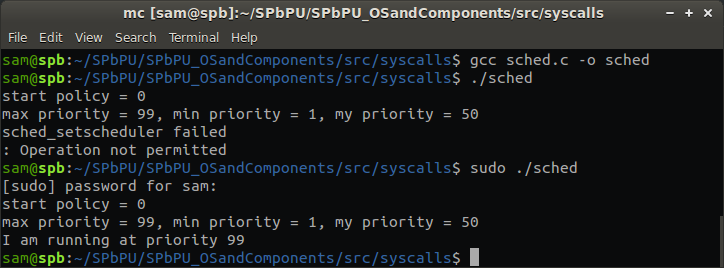
\includegraphics[scale=0.7]{res/pic002}
\caption{Результат запуска программы sched}
\end{figure}

Для отслеживания системных вызовов будем использовать strace. Эта утилита отслеживает системные вызовы и представляют собой механизм трансляции, обеспечивающий интерфейс между процессом и операционной системой (ядром). Эти вызовы могут быть перехвачены и прочитаны, что позволяет лучше понять, что процесс пытается сделать в заданное время. Перехватывая эти вызовы, можно добиться лучшего понимания поведения процессов, особенно в процессе отладки. Функциональность операционной системы, позволяющая отслеживать системные вызовы, называется ptrace. Strace вызывает ptrace и читает данные о поведении процесса, возвращая отчет.

Отчёт по работе программы sched представлен в листинге 2.

\lstinputlisting[language={},caption={Протокол системных вызовов}]{res/strace.rep}

Как можно видеть в листинге 2, помимо изучаемых программа делает ещё множество стронних вызовов (к примеру, подгружает системные библиотеки). Но в последних строчках просисходят ожидаемые системные вызовы. % Использование системных вызовов из пользовательского кода



\newpage
\section*{}
\addcontentsline{toc}{section}{Список литературы}

\begin{thebibliography}{00}

\bibitem{Love} Роберт Лав: «Разработка ядра Linux», Вильямс, 448 стр., 2008, ISBN
5-8459-1085-1, 0-672-32720-1.

\bibitem{Cragon} Harvey G. Cragon: «Computer Architecture and Implementation», Cambridge University Press, 238 pages, 2000, ISBN-10: 521651689.

\bibitem{Rosen} Rami Rosen: «Linux Kernel Networking: Implementation and Theory», Apress, 650 pages, 2014, ISBN-13: 978-1-4302-6196-4.

\bibitem{Realtech} Realtech: RTL8111B, Single-Chip Gigabit LOM Ethernet Controller for PCI Express. Datasheet Rev. 1.4, 02 December 2005, Track ID: JATR-1076-21.

\end{thebibliography} % Источники

%------------------------------------------------------------------------------

\end{document}